We compare the performance of 3 memory management strategies 
\begin{description}
\item[\none] -- which does no compaction of the data, this was previously the default in HBase.
\item[\basic] -- which reduces the representation of the index, this is the default in HBase 2.0.
\item[\magic] -- which compact both the data and index and is adaptive to the workload behavior, this is still an experimental feature.
\end{description}

We compare the strategies by measuring their throughput and latency. In addition we measure the write volume, that is the number of KB written to the file system, and the cumulative gc time of each run.
We also compare different setting of the same strategy in order to find the optimal configuration.

\paragraph{Experiment setup.}

Our experiments run on 2  clusters with different hardware. 
The first cluster consists of five 12-core Intel Xeon 5 machines with 46GB RAM and 4TB 
SSD storage, interconnected by 1G Ethernet. 
The second cluster consists of five 8-core 
Intel Xeon E5620 servers with 24GB RAM and 1TB magnetic drive. The interconnects  are 1Gbps Ethernet. 
We denote these clusters as the SSD cluster and HDD cluster, respectively.
In both clusters we allocate three nodes to HBase nodes, 1 master and 2 region servers, one to simulate the client whose performance we measure, and one to simulate background traffic
as explained below. Each HBase node runs both an HBase region server or master within 8GB JVM containers and the underlying 
Hadoop File System (HDFS) server . 

The traffic is driven by a client running the popular YCSB benchmark~\cite{Cooper}. 
We run write-only and mixed read-write workload where keys are chosen either from either a zipfian or uniform distribution over 100 millions keys.
In all the experiments we create a table with 4 columns (in a single column family). Each update operation writes 25 Bytes values to all 4 columns of a single key, namely writing 100 Bytes of data.


\paragraph{GC overhead.}

Our experiment show that in write-only workloads gc and throughput have a very high correlation. 
Figure~\ref{fig:gc-throughput-log2} plots the scatter graph of cumulative gc time vs write throughput of several write-only experiments of the system with varying settings in different strategies. It clearly shows that  the lower the gc overhead is, the higher the throughput is.
Specifically, there is a negative linear correlation between their values on a log-log scale.

\begin{figure}[htb]
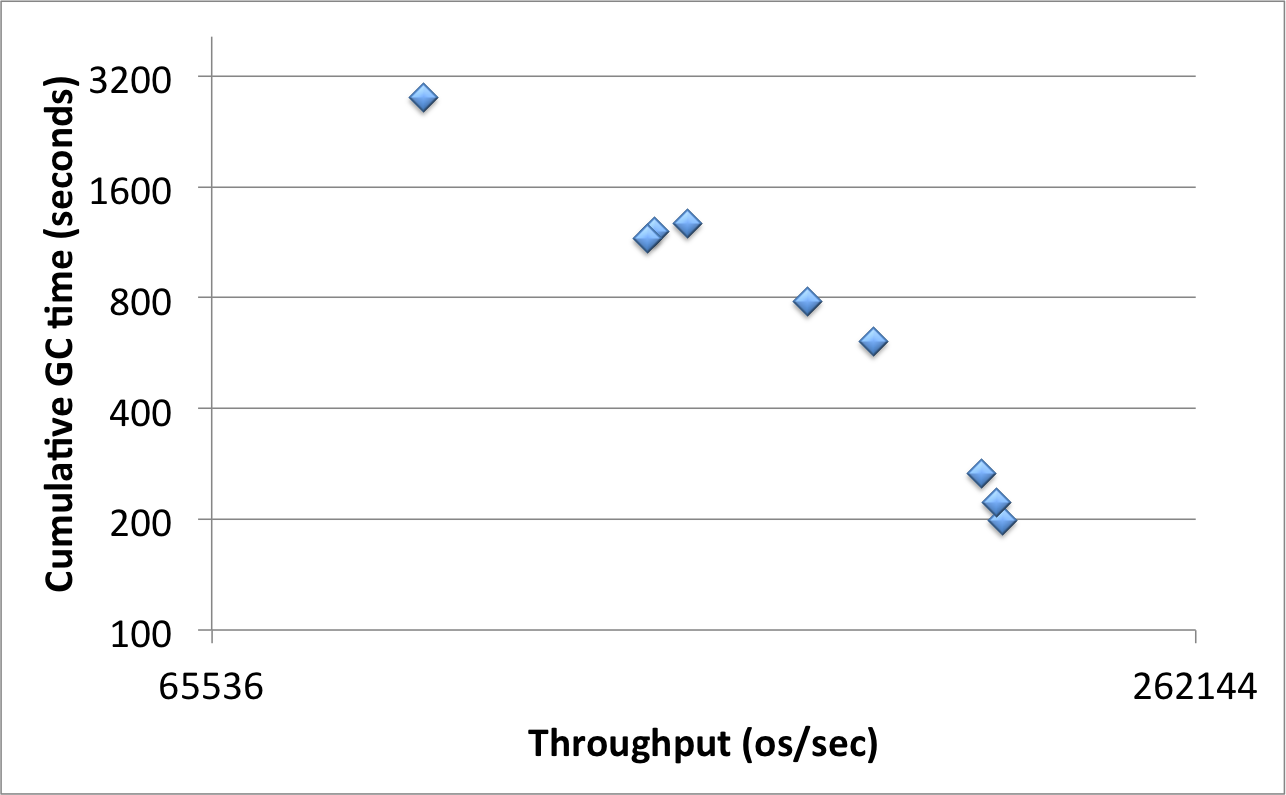
\includegraphics[width=\figw]{Figs/gc-throughput-log2.png}
\caption{{\bf GC-Throughput correlation.} Log-log scale plot of the cumulative gc time vs write throughput in different settings shows negative linear correlation.
}
\label{fig:gc-throughput-log2}
\end{figure}